\documentclass{IEEEtran}
\usepackage{cite}
\usepackage{amsmath,amssymb,amsfonts}
\usepackage{graphicx}
\usepackage{textcomp,nicefrac}

%-----------------------------------------------------------------------------------
\usepackage{algorithmicx}
\usepackage{algpseudocode}

% define float env for algorithm
\usepackage{float}
\floatstyle{ruled}
\newfloat{algorithm}{h}{loa}
\floatname{algorithm}{Algorithm}

% custom definitions
\DeclareMathOperator{\proj}{proj}
\DeclareMathOperator{\prox}{prox}
\DeclareMathOperator*{\argmin}{arg\,min}
%-----------------------------------------------------------------------------------


\def\BibTeX{{\rm B\kern-.05em{\sc i\kern-.025em b}\kern-.08em
T\kern-.1667em\lower.7ex\hbox{E}\kern-.125emX}}
\markboth{IEEE NSS/MIC conference 2021}
{Schramm \MakeLowercase{\textit{et al.}}: List-mode SPDHG}

\begin{document}
\title{Fast list-mode reconstruction of sparse TOF PET data with non-smooth priors} 
\author{Georg Schramm and Martin Holler
\thanks{G.S. is with the Department of Imaging and Pathology, Division of Nuclear Medicine,
KU Leuven, Belgium, (e-mail: georg.schramm@kuleuven.be).}
\thanks{M.H. is with the Institute of Mathematics and Scientific Computing, 
University of Graz, Austria}
}

\maketitle

\begin{abstract}
In this work, we propose and analyze a list-mode version of the stochastic primal-dual hybrid gradient
(SPDHG) algorithm which (i) substantially reduces its memory requirements and (ii) reduces
computation time when reconstruction sparse TOF PET data using subsets and non-smooth priors. 
To study the behavior of the proposed algorithm in detail, its performance 
is investigated based on simulated 2D TOF data using a brain-like software phantom.

We find that listmode-version of SPDHG converges almost as fast the original version
which will lead to a substantial improvement in the time needed for a reconstruction
of real 3D TOF PET data.
However, a careful choice of the ratio of the primal and dual step sizes, 
depending on the magnitude of the image to be reconstructed, is crucial to obtain fast convergence.
\end{abstract}

\begin{IEEEkeywords}
Positron emission tomography, Reconstruction algorithms
\end{IEEEkeywords}

\section{Introduction}
foo bar

\section{Methods}

%-----------------------------------------------------------------------------
\begin{algorithm}[t]
\begin{algorithmic}[1]
\footnotesize
\State \textbf{Initialize} $x,(S_i)_i,T,(p_i)_i,g$
\State \textbf{Calculate} event counts $\mu_e$ for each e in $N$
\State \textbf{Split} event list $N$ into $m$ sublists $N_i$
\State \textbf{Initialize} $m$ sub lists $l_{N_i}$ with 0s
\State \textbf{Preprocessing} $\overline{z} = z = P^T y$ where $y$ is XXX
\Repeat
	\State $x = \proj_{\geq 0} (x - T \overline{z})$
	\State Select $i \in \{1,\ldots,m+1\}$ randomly accord. to $(p_i)_i$
  \If{$i \leq m$}
	  \State $l_{N_i}^+ \gets \prox_{D^*}^{S_i} \left( l_{N_i} + S_i \left(P_{N_i} x + s_{N_i} \right) \right)$
	  \State $\delta z \gets P_{N_i}^T \left(\frac{l_{N_i}^+ - l_{N_i}}{\mu_{N_i}}\right)$
	  \State $l_{N_i} \gets l_{N_i}^+$
  \Else
	  \State $g^+ \gets \prox_{N^*}^{S_i} \left( g + S_i \nabla x \right)$
	  \State $\delta z \gets \nabla^T \left(g^+ - g\right)$
	  \State $g \gets g^+$
  \EndIf
	\State $z \gets z + \delta z$
	\State $\overline{z} \gets  z + (\delta z/p_i)$
\Until{stopping criterion fulfilled}
\State \Return{$x$}
%\EndFunction
\end{algorithmic}
\caption{List-mode SPDHG for PET reconstruction}
\label{alg:spdhg}
\end{algorithm}
%-----------------------------------------------------------------------------

\begin{figure}[t]
\centerline{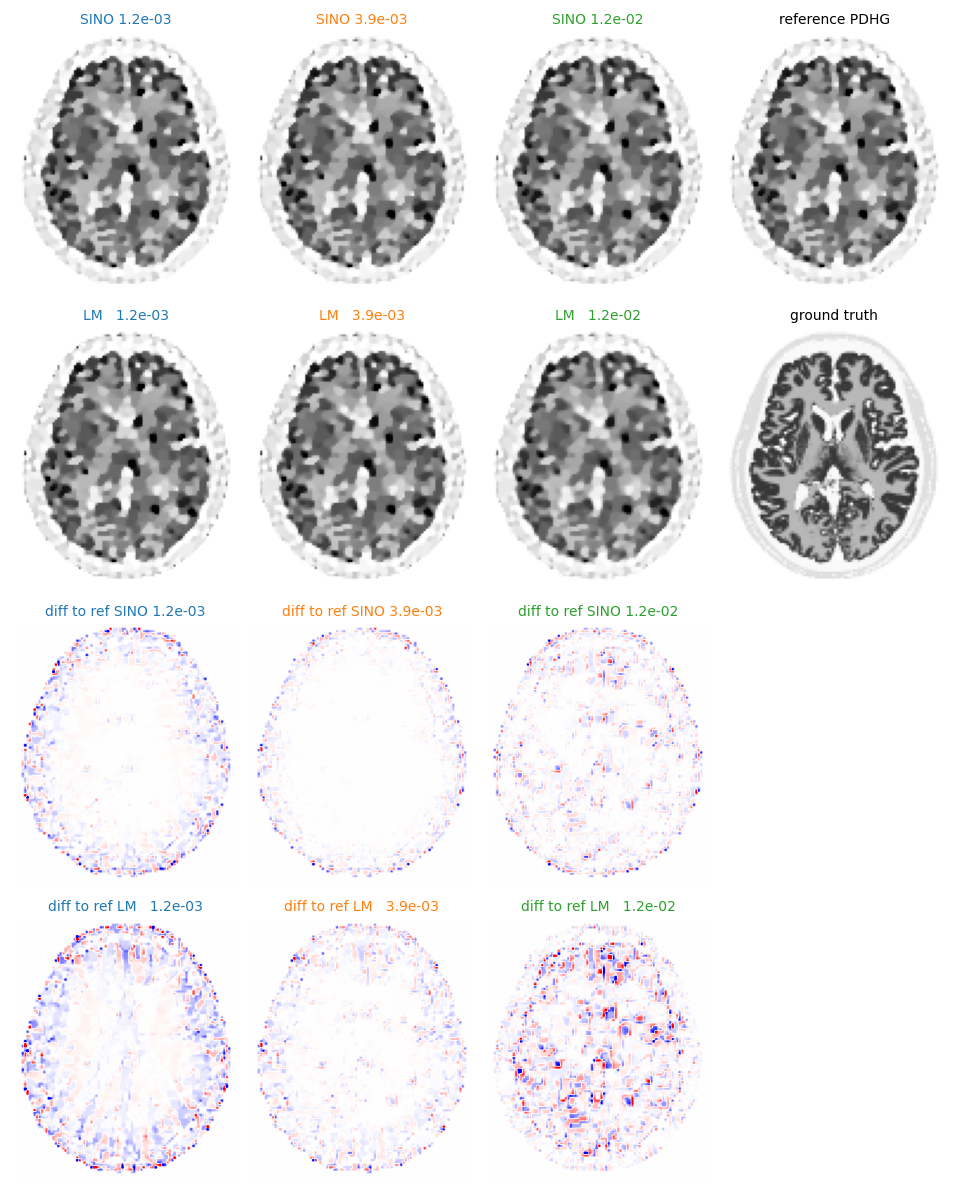
\includegraphics[width=1.0\columnwidth]{./figs/brain2d_counts_1.0E+06_beta_2.0E-03_niter_5000_100_nsub_56_precond_False.png}}
\caption{foo bar}
\label{fig:recons}
\end{figure}

\begin{figure}[t]
\centerline{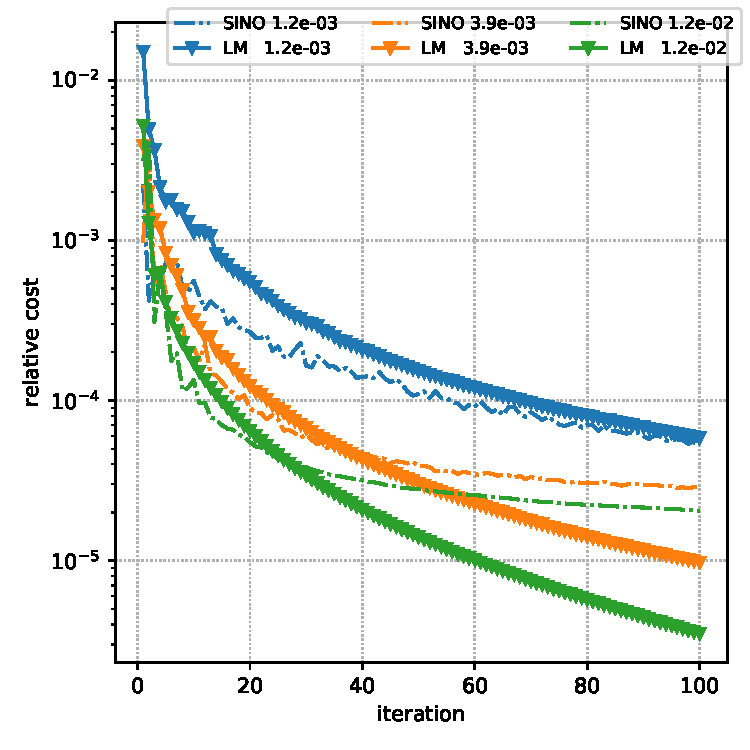
\includegraphics[width=0.7\columnwidth]{./figs/brain2d_counts_1.0E+06_beta_2.0E-03_niter_5000_100_nsub_56_precond_False_metrics.pdf}}
\caption{foo bar}
\label{fig:cost}
\end{figure}



%\section{Introduction}
%\label{sec:introduction}
%\IEEEPARstart{T}{his} document is a template for \LaTeX. If, after reading these
%instructions, you still have questions or require assistance, please contact
%\underline {tns-editor@ieee.org}. If you are
%reading a paper or PDF version of this document, please download the
%electronic file, trans\_jour.tex, from the IEEE Web site at \underline
%{http://www.ieee.org/authortools/trans\_jour.tex} so you can use it
%to prepare your manuscript. You can also explore using the Overleaf editor at
%\underline{https://www.overleaf.com/blog/278-how-to-use-overleaf-with-}\discretionary{}{}{}\underline
%{ieee-collabratec-your-quick-guide-to-getting-started\#.}\discretionary{}{}{}\underline{xsVp6tpPkrKM9}
%Your submitted paper should be
%in this 2-column format with figures and tables embedded in the text.
%
%The general IEEE policy requires that authors should only submit original
%work that has neither appeared elsewhere for publication, nor is under
%review for another refereed publication. The submitting author must disclose
%to the editor if any part of the manuscript has been previously published or
%submitted for publication elsewhere when submitting a manuscript. Do not
%submit ``preliminary'' data or results.
%
%The submitting author is responsible for obtaining agreement of all
%coauthors and any consent required from employers or sponsors before
%submitting an article. The submitting author is also responsible for
%obtaining permission from the copyright holder to republish copyrighted
%material. Transactions on Nuclear Science (TNS) strongly discourages
%courtesy authorship. It is the obligation of the authors to cite relevant
%prior work and only relevant prior work.
%
%TNS does not publish conference records or proceedings, but can publish
%articles related to conferences after they have undergone rigorous peer
%review. Articles that have already appeared in an unreferred conference
%proceeding (or other medium) and that include a substantial amount
%($>50\%$) of new information may be acceptable.
%
%All papers submitted to TNS undergo peer review and an automated plagiarism
%check. Papers failing the plagiarism check will be rejected without further
%review. Every published article receives a minimum of two independent
%reviews.
%
%Articles for peer-review can be submitted at any time, and are generally 8
%pages in length, including figures, tables, equations, and references. TNS
%also publishes tutorial expositions and critical reviews, however, we ask
%that authors contact the editor in chief prior to submitting such a work.
%
%Authors should consider the following points:
%
%\begin{enumerate}
%\item Technical papers submitted for publication must advance the state of knowledge and must cite relevant prior work. An obvious or minor extension of previously published work might not be appropriate for publication.
%\item Authors must convince both peer reviewers and the editors of the scientific and technical merit of a paper; the standards of proof are higher when extraordinary or unexpected results are reported.
%\item Because replication is required for scientific progress, papers submitted for publication must provide sufficient information to allow readers to perform similar experiments or calculations and use the reported results. Although not everything need be disclosed, a paper must contain new, useable, and fully described information. For example, a specimen's chemical composition need not be reported if the main purpose of a paper is to introduce a new measurement technique. However, if that composition is critical to the technique, then it should be disclosed. Authors should expect to be challenged by reviewers if the results are not supported by adequate data and critical details.
%\item Papers that describe ongoing work or announce the latest technical achievement, which are suitable for presentation at a professional conference, generally are not appropriate for TNS.
%\end{enumerate}
%
%Additional information on the requirements for the technical content of
%manuscripts of manuscripts submitted to TNS and on its review process,
%including scope, content, and items for authors to address in their articles
%are available at \underline
%{https://}\discretionary{}{}{}\underline{ieee-npss.org/publications/transactions-on-nuclear-science/}.
%
%\section{Structure of your paper}
%Your paper will consist of at least four sections: an Introduction, a
%description of the measurement, theory, computation, equipment, etc., a
%discussion of the data and analysis, and a set of conclusions drawn from the
%data and analysis. Feel free to add additional sections as necessary.
%
%The Introduction motivates the work. Explain here why it is important, what
%deficiencies in the state of the art you aim to overcome, how/why the work
%extends the state of the art. Describe the problem you are trying to solve.
%Include a review of relevant literature in this section.
%
%In the Experimental section, you describe your equipment, technique,
%materials, protocols, and whatever else is necessary so that another person
%working in your field can understand what you did and reproduce the work.
%
%Discuss the data you acquired and how you analyzed them. Include a
%statistical analysis to demonstrate the limits of the data analysis.
%Experimental data have uncertainties, although the error bars may be smaller
%than the symbols used to represent them. Your discussion should include
%something about the experimental uncertainties. Even simulations have (or
%can have) uncertainties associated with them. TNS expects to see a
%discussion of uncertainties in all papers.
%
%A Conclusions (note the plural) section is required. Although this section
%may review the main points of the paper, do not replicate the abstract here.
%A Conclusions section draws inferences from the data and elaborates on the
%importance of the work. You may suggest applications and extensions. You
%should explain here how the data and analysis support the introduction to
%your paper where you motivated and justified the work. Explain how the work
%extends the state of the art. Answer the question ``So what?''
%
%\subsection{Abbreviations and Acronyms}
%Define abbreviations and acronyms the first time they are used in the text,
%even after they have already been defined in the abstract. Common
%abbreviations such as IEEE, SI, ac, and dc do not have to be defined.
%Abbreviations that incorporate periods should not have spaces: write
%``C.N.R.S.,'' not ``C. N. R. S.'' Do not use abbreviations in the title
%unless they are unavoidable (for example, ``IEEE'' in the title of this
%article).
%
%\subsection{Inclusion of copyrighted material}
%Sometimes it is expedient to include a figure, table, equation, or text from
%a previously published work. If you find it useful to do this, it is your
%responsibility to obtain permission from the copyright holder (usually the
%publisher of the work. You must indicate the items in your paper that have
%been reproduced from prior work and include a reference to the source of the
%material in the references. Captions of reproduced figures and tables should
%include ``Reproduced from [nnn], with permission.'' or whatever the
%copyright holder requires. Reproduced text should be offset from the body of
%your paper, enclosed in quotation marks, and include the permission
%statement as for figures and tables.
%
%\subsection{Other Recommendations}
%Use one space after periods and colons. Hyphenate complex modifiers:
%``zero-field-cooled magnetization.'' Avoid dangling participles, such as,
%``Using (\ref{eq1}), the potential was calculated.'' [It is not clear who or what
%used (\ref{eq1}).] Write instead, ``The potential was calculated by using (\ref{eq1}),'' or
%``Using (\ref{eq1}), we calculated the potential.''
%
%Use a zero before decimal points: ``0.25,'' not ``.25.'' Indicate sample
%dimensions as ``$0.1~\text{cm} \times 0.2~\text{cm}$,'' not ``$0.1
%\times 0.2~\text{cm}^{2}$.'' The abbreviation for ``seconds'' is ``s,'' not ``sec.'' Do not
%mix abbreviations and full names of units. Write m/s, not meters/s. When
%expressing a range of values, write ``7 to 9'' or ``7--9,'' and not
%``$7\sim9$'' or ``$7\div 9$.'' Note that periods (.) and commas
%(,) are punctuated within the quotation marks.
%
%A parenthetical statement at the end of a sentence is punctuated outside of
%the closing parenthesis (like this). (A parenthetical sentence is punctuated
%within the parentheses.) In US English, periods and commas are within
%quotation marks, like ``this period.'' Other punctuation is ``outside''!
%Avoid contractions; for example, write ``do not'' instead of ``don't.'' The
%serial comma is preferred: ``A, B, and C'' instead of ``A, B and C.''
%
%If you wish, you may write in the first person singular or plural and use
%the active voice (``I observed that \textellipsis'' or ``We observed that \textellipsis''
%instead of ``It was observed that \textellipsis''). Remember to check spelling. If
%your native language is not English, please ask a native English-speaking
%colleague, a teacher of English as a second language, or a professional
%translation service to proofread your paper carefully. Papers may be
%rejected without review if the English usage is unsatisfactory. TNS prefers
%US spelling (color rather than colour).
%
%Try not to use too many typefaces in the same article. You're writing
%scholarly papers, not ransom notes. Also please remember that MathJax
%can't handle really weird typefaces.
%
%\subsection{Equations}
%Number equations consecutively with equation numbers in parentheses flush
%with the right margin, as in (\ref{eq1}). First use the equation editor to create
%the equation. Then select the ``Equation'' markup style. Press the tab key
%and write the equation number in parentheses. To make your equations more
%compact, you may use the solidus (~/~), the exp function, or appropriate
%exponents. Use parentheses to avoid ambiguities in denominators. Punctuate
%equations when they are part of a sentence, as in
%\begin{equation}
%\label{eq1}
%x=\frac{111111111}{12345679}=9 .
%\end{equation}
%Note that $x$ is math mode because it is a variable. Be sure that the symbols
%in your equation have been defined before the equation appears or
%immediately following. Symbols must be in math mode, but not units: $T$ referring to
%temperature, but T as the unit tesla. Refer to ``(\ref{eq1}),'' not ``Eq. (\ref{eq1})'' or
%``equation (\ref{eq1}),'' except at the beginning of a sentence: ``Equation (\ref{eq1}) is
%{\textellipsis}~.''
%
%\subsection{\LaTeX-Specific Advice}
%
%Please use ``soft'' (e.g., \verb|\eqref{Eq}|) cross references instead
%of ``hard'' references (e.g., \verb|(1)|). That will make it possible
%to combine sections, add equations, or change the order of figures or
%citations without having to go through the file line by line.
%
%Please don't use the \verb|{eqnarray}| equation environment. Use
%\verb|{align}| or \verb|{IEEEeqnarray}| instead. The \verb|{eqnarray}|
%environment leaves unsightly spaces around relation symbols.
%
%Please note that the \verb|{subequations}| environment in {\LaTeX}
%will increment the main equation counter even when there are no
%equation numbers displayed. If you forget that, you might write an
%article in which the equation numbers skip from (17) to (20), causing
%the copy editors to wonder if you've discovered a new method of
%counting.
%
%{\BibTeX} does not work by magic. It doesn't get the bibliographic
%data from thin air but from .bib files. If you use {\BibTeX} to produce a
%bibliography you must send either the .bbl file or the .bib files.
%If you use \texttt{biblatex}, please send the .bib file. The .bbl file
%generated by \texttt{biblatex} is not designed to be edited.
%
%{\LaTeX} can't read your mind. If you assign the same label to a
%subsubsection and a table, you might find that Table I has been cross
%referenced as Table IV-B3.
%
%{\LaTeX} does not have precognitive abilities. If you put a
%\verb|\label| command before the command that updates the counter it's
%supposed to be using, the label will pick up the last counter to be
%cross referenced instead. In particular, a \verb|\label| command
%should not go before the caption of a figure or a table.
%
%Do not use \verb|\nonumber| or \verb|\notag| inside the \verb|{array}| environment. It
%will not stop equation numbers inside \verb|{array}| (there won't be
%any anyway) and it might stop a wanted equation number in the
%surrounding equation.
%
%\section{Units}
%Use either SI (MKS) or CGS as primary units. (SI units are strongly
%encouraged.) English units may be used as secondary units (in
%parentheses). This applies to papers discussing data storage, also.
%For example, write ``15 Gb/cm$^{2}$ (100 Gb/in$^{2})$.'' An exception
%is when English units are used as identifiers in trade, such as
%``$3\nicefrac{1}{2}$-in disk drive.'' Avoid combining SI and CGS units,
%such as density in kg/cm$^{3}$ because this can lead to confusion when
%equations do not balance dimensionally. If you must use mixed units,
%clearly state the units for each quantity in an equation.
%
%The SI unit for magnetic field strength $H$ is A/m. However, if you wish to use
%units of T, either refer to magnetic flux density $B$ or magnetic field
%strength symbolized as $\mu _{0}H$. Use the center dot to separate
%compound units, e.g., ``$\text{A}\cdot \text{m}^{2}$.''
%
%\section{Guidelines for Graphics Preparation}
%Tables, graphs, charts, and images should be embedded in the text of your
%paper rather than collected in pages after the text. They should be
%mentioned on the same page or before the appearance of the object itself, as
%\figurename~\ref{fig1} is mentioned here. If there is insufficient
%room in a column for a figure, rather than compress it, the figure is
%allowed to move to the next page and white space is left immediately below.
%Alternatively, you can move text from below the figure to this space, if it
%makes sense to do so. It is good practice to tell the reader what is in the
%figure in the caption and you can include a sentence or two about the
%significance of the figure in the caption. However, lengthy explanations
%should be placed in the body of the paper.
%
%\begin{figure}[t]
%\centerline{\includegraphics[width=3.5in]{tns1.png}}
%\centerline{\includegraphics[width=3.5in]{tns2.png}}
%\caption{Differential (a) and integral probability of interaction as a function of
%angle of incidence.}
%\label{fig1}
%\end{figure}
%
%\subsection{Multipart figures}
%Figures comprising more than one sub-figure are presented side-by-side, or
%stacked. Add an alphabetic label enclosed in parentheses inside each
%sub-figure: (a), (b), (c), {\textellipsis}~. Choose a color for the text so
%that it is visible over the image. The text box containing the label should
%have no fill or border; only the letter in parentheses should be visible.
%
%The figure caption will identify each sub-figure it is describing with these
%labels. Write ``(a) Differential probability of interaction.
%(b) Integral probability of interaction, both as a function of angle of
%incidence,'' or ``Differential (a) and integral (b) probability of
%interaction as a function of angle of incidence.'' Refer to the sub-figure as
%\figurename~\ref{fig1}a in the body of the text.
%
%If you choose to place figures (multipart or not) side-by-side in a single
%column you might find it convenient to insert them in a single row of a
%tabular. You can then place the captions in next row or insert them in the
%same cell as the figure to keep the captions aligned with the figures.
%
%\subsection{Using Labels Within Figures}
%When preparing your graphics, if you prefer them to match the text of
%the article, IEEE suggests that you use Times New Roman. The example
%uses Cambria. (This guideline was originally written for \emph{Word}.)
%
%Figure axis labels are often a source of confusion. Use words rather than
%symbols. As an example, write the quantity ``Angle,'' and the units in
%parentheses. Do not label axes only with units. Thus ``Angle of incidence
%($^{\circ}$)'' and not just ``$^{\circ}$,''in Fig. 1, above. Do not
%label axes as a ratio of quantities and units. For example, write
%``Temperature (K),'' not ``Temperature/K.''
%
%Multipliers can be especially confusing. Write ``Distance (m)'' or
%``Distance (km).'' Do not write ``Distance (m) $\times$ 1000'' because the
%reader would not know whether the tick mark labels have already been
%multiplied by 1000 or whether the reader needs to multiply them by 1000.
%Similarly, do not put a multiplier at the end of an axis. Figure labels must
%be legible; use at least 8- to 10-point type.
%
%\subsection{Tables}
%Tables are inserted as {\LaTeX} tables, not as images, and should also be mentioned
%in advance of their appearance. Table~\ref{tab1} shows an
%acceptable layout of a table having both supplementary information below the
%table and an internal footnote. The explanation of the footnote appears
%after the supplementary information.
%
%\begin{table}
%\caption{Units for Magnetic Properties}
%\label{table}
%\setlength{\tabcolsep}{3pt}
%\begin{tabular}{|p{25pt}|p{75pt}|p{115pt}|}
%\hline
%Symbol&
%Quantity&
%Conversion from Gaussian and \par CGS EMU to SI $^{\mathrm{a}}$ \\
%\hline
%$\Phi $&
%magnetic flux&
%1 Mx $\to 10^{-8}$ Wb $= 10^{-8}$ V$\cdot $s \\
%$B$&
%magnetic flux density, \par magnetic induction&
%1 G $\to 10^{-4}$ T $= 10^{-4}$ Wb/m$^{2}$ \\
%$H$&
%magnetic field strength&
%1 Oe $\to 10^{3}/(4\pi )$ A/m \\
%$m$&
%magnetic moment&
%1 erg/G $=$ 1 emu \par $\to 10^{-3}$ A$\cdot $m$^{2} = 10^{-3}$ J/T \\
%$M$&
%magnetization&
%1 erg/(G$\cdot $cm$^{3}) =$ 1 emu/cm$^{3}$ \par $\to 10^{3}$ A/m \\
%4$\pi M$&
%magnetization&
%1 G $\to 10^{3}/(4\pi )$ A/m \\
%$\sigma $&
%specific magnetization&
%1 erg/(G$\cdot $g) $=$ 1 emu/g $\to $ 1 A$\cdot $m$^{2}$/kg \\
%$j$&
%magnetic dipole \par moment&
%1 erg/G $=$ 1 emu \par $\to 4\pi \times 10^{-10}$ Wb$\cdot $m \\
%$J$&
%magnetic polarization&
%1 erg/(G$\cdot $cm$^{3}) =$ 1 emu/cm$^{3}$ \par $\to 4\pi \times 10^{-4}$ T \\
%$\chi , \kappa $&
%susceptibility&
%1 $\to 4\pi $ \\
%$\chi_{\rho }$&
%mass susceptibility&
%1 cm$^{3}$/g $\to 4\pi \times 10^{-3}$ m$^{3}$/kg \\
%$\mu $&
%permeability&
%1 $\to 4\pi \times 10^{-7}$ H/m \par $= 4\pi \times 10^{-7}$ Wb/(A$\cdot $m) \\
%$\mu_{r}$&
%relative permeability&
%$\mu \to \mu_{r}$ \\
%$w, W$&
%energy density&
%1 erg/cm$^{3} \to 10^{-1}$ J/m$^{3}$ \\
%$N, D$&
%demagnetizing factor&
%1 $\to 1/(4\pi )$ \\
%\hline
%\multicolumn{3}{p{251pt}}{Vertical lines are optional in tables. Statements that serve as captions for
%the entire table do not need footnote letters. }\\
%\multicolumn{3}{p{251pt}}{$^{\mathrm{a}}$Gaussian units are the same as cg emu for magnetostatics; Mx
%$=$ maxwell, G $=$ gauss, Oe $=$ oersted; Wb $=$ weber, V $=$ volt, s $=$
%second, T $=$ tesla, m $=$ meter, A $=$ ampere, J $=$ joule, kg $=$
%kilogram, H $=$ henry.}
%\end{tabular}
%\label{tab1}
%\end{table}
%
%\subsection{Referring to a Figure or Table Within Your Paper}
%\label{subsec:referring}
%When referring to your figures and tables within your paper, use the
%abbreviation ``Fig.'' even at the beginning of a sentence. Do not abbreviate
%``Table.''
%
%It is best if tables do not span pages and columns, but sometimes that
%cannot be helped. When a table must span a page, please repeat the column
%headings on each page.
%
%\subsection{Sizing of Graphics}
%Most charts, graphs, and tables are one column wide (3.5 inches~/ 88
%millimeters~/ 21 picas) or page wide (7.16 inches~/ 181 millimeters~/ 43
%picas). The maximum height a graphic can be is 8.5 inches (216 millimeters~/
%54 picas). When choosing the height of a graphic, please allow space for a
%caption. Figures can be sized between column and page widths if the author
%chooses, however it is recommended that figures are not sized less than
%column width unless necessary.
%
%\subsection{File Formats For Graphics}\label{formats}
%Format and save your graphics using a suitable graphics processing program
%that will allow you to create the images as PostScript (PS), Encapsulated
%PostScript (.EPS), Tagged Image File Format (.TIFF), Portable Document
%Format (.PDF), Portable Network Graphics (.PNG), or Metapost (.MPS), sizes them, and adjusts
%the resolution settings. When
%submitting your final paper, your graphics should all be submitted
%individually in one of these formats along with the manuscript.
%
%\section{Some Common Misteaks}
%Always check your spelling. The word ``data'' is plural, not singular; the
%singular is ``datum.'' Use the word ``micrometer'' instead of ``micron,'' or
%write ``$\mu $m.'' A graph within a graph is an ``inset,'' not an
%``insert.'' The word ``alternatively'' is preferred to the word
%``alternately'' (unless you really mean something that alternates). Use the
%word ``whereas'' instead of ``while'' (unless you are referring to
%simultaneous events). Do not use the word ``essentially'' to mean
%``approximately'' or ``effectively.'' Do not use the word ``issue'' as a
%euphemism for ``problem.'' When compositions are not specified, separate
%chemical symbols by en-dashes; for example, ``NiMn'' indicates the intermetallic
%compound Ni$_{0.5}$Mn$_{0.5}$ whereas \text{``Ni--Mn''} indicates an alloy of some
%composition Ni$_{x}$Mn$_{1-x}$.
%
%Be aware of the different meanings of the similar words ``affect'' (usually
%a verb) and ``effect'' (usually a noun), ``complement'' and ``compliment,''
%``discreet'' and ``discrete,'' ``principal'' (e.g., ``principal
%investigator'') and ``principle'' (e.g., ``principle of measurement''). Do
%not confuse ``imply'' and ``infer.'' Data imply something; people infer
%something from the data.
%
%Prefixes such as ``non,'' ``sub,'' ``micro,'' ``multi,'' and ``ultra'' are
%not independent words when used as modifiers; they should be joined to the
%words they modify, usually, but not exclusively, without a hyphen:
%nonuniform, subminiature, micrometer, multimeter, ultrasound. However, if
%your paper needs to mention a submarine, TNS prefers you write out the word
%rather than use the word ``sub.'' There is no period after the ``et'' in the
%Latin abbreviation ``\textit{et al.}'' (it is the italicized abbreviation for \textit{et alia,} meaning
%``and others''). The abbreviation ``i.e.'' abbreviates \textit{id est}, meaning ``that
%is,'' and ``e.g.'' abbreviates the Latin \textit{exempli gratia}, meaning ``for example.'' These
%last two abbreviations are \textit{not} italicized).
%
%Please do not use math mode for italicized text.
%
%\section{Conclusion}
%The manuscript submitted to TNS for consideration for publication should be
%formatted according to this document. Doing so will allow an efficient
%review process and minimize the effort required by authors in preparing
%their final files, if the manuscript is accepted for publication.
%
%Key factors to consider include the following:
%
%\begin{itemize}
%\item The document must be in this two-column format.
%\item Font sizes for text, section headings, etc. must conform to those in this template.
%\item Proper English usage is necessary. Manuscripts which are vague or unclear because of poor grammar or wording may be rejected without review.
%\item The nominal maximum page length for the submitted manuscript is 8 pages, unless prior arrangements are made with the editor to accept a longer submission.
%\end{itemize}
%
%\appendices
%
%\section*{Appendix}
%
%Appendixes, if needed, appear before the acknowledgment. They do not have
%Roman numeral section numbers. Use
%the \verb|\appendices| command for multiple appendices and
%\verb|\appendix| for a single appendix. Do not use \verb|\section|
%inside a single Appendix.
%
%If you prefer to number equations separately in each Appendix, please
%use \verb|\numberwithin{equation}{section}| instead of redefining
%equation macros or resetting the equation counter.
%
%\section*{Acknowledgment}
%
%Acknowledgments, if any, appear after any appendices and before the list of
%references. The preferred spelling of the word ``acknowledgment'' in US
%English is without an ``e'' after the ``g.'' Use the singular heading even
%if you have many acknowledgments. Avoid expressions such as ``One of us
%(S.B.A.) would like to thank \textellipsis~.'' Instead, write ``F. A. Author thanks
%\textellipsis~.'' In most cases, sponsor and financial support acknowledgments are
%placed in the unnumbered footnote on the first page, not here.
%
%\section*{References and Footnotes}
%
%\subsection{References}
%References need not be cited in text. When they are, they appear on the
%line, in square brackets, inside the punctuation. Multiple references are
%each numbered with separate brackets. When citing a section in a book,
%please give the relevant page numbers. In text, refer simply to the
%reference number. Do not use ``Ref.'' or ``reference'' except at the
%beginning of a sentence: ``Reference \cite{b3} shows \textellipsis~.''
%
%Please us the standard reference format in which
%reference numbers are set flush left and form a column of their own, hanging
%out beyond the body of the reference. The reference numbers are on the line,
%enclosed in square brackets. In all references, the given name of the author
%or editor is abbreviated to the initial only and precedes the last name. Use
%them all; use \emph{et al.} only if names are not given. Use commas around Jr.,
%Sr., and III in names. Abbreviate conference titles. When citing IEEE
%transactions, provide the issue number, page range, volume number, year,
%and/or month if available. When referencing a patent, provide the day and
%the month of issue, or application. References may not include all
%information; please obtain and include relevant information. Do not combine
%references. There must be only one reference with each number. If there is a
%URL included with the print reference, it can be included at the end of the
%reference.
%
%Other than books, capitalize only the first word in a paper title, except
%for proper nouns and element symbols. For papers published in translation
%journals, please give the English citation first, followed by the original
%foreign-language citation See the end of this document for formats and
%examples of common references. For a complete discussion of references and
%their formats, see the IEEE style manual at
%\underline{http://www.ieee.org/authortools}.
%
%\subsection{Footnotes}
%Other than the unnumbered affiliations footnote on page 1 of your paper, do
%not use footnotes in your paper. Information that might go in a footnote can
%become a parenthetical phrase or sentence or just be incorporated into the
%text.
%
%\section*{References}
%
%\def\refname{\vadjust{\vspace*{-1em}}} %Please don't do this in a real paper.
%
%\subsection*{Basic format for books:}
%
%\begin{thebibliography}{00}
%\bibitem{b1} J. K. Author, ``Title of chapter in the book,'' in \textit{Title of His Published Book, x}th ed. City of Publisher,
%(only U.S. State), Country: Abbrev. of Publisher, year, ch. x, sec. x, pp.
%\textit{xxx--xxx.}
%\end{thebibliography}
%
%\subsection*{Examples:}
%
%\begin{thebibliography}{00}
%\bibitem{b2} G. O. Young, ``Synthetic structure of industrial
%plastics,'' in \emph{Plastics}, 2nd ed., vol. 3, J. Peters, Ed. New York, NY, USA: McGraw-Hill, 1964, pp. 15--64.
%\bibitem{b3} W.-K. Chen, \emph{Linear Networks and Systems}. Belmont, CA, USA: Wadsworth, 1993, pp. 123--135.
%\end{thebibliography}
%
%\subsection*{Basic format for periodicals:}
%
%\begin{thebibliography}{00}
%\bibitem{b4} J. K. Author, ``Name of paper,'' \textit{Abbrev. Title of Periodical}, vol. x, no. x, pp. xxx-xxx, Abbrev. Month, year, DOI.
%10.1109.\textit{XXX}.123456.
%\end{thebibliography}
%
%\subsection*{Examples:}
%
%\begin{thebibliography}{00}
%\bibitem{b5} J. U. Duncombe, ``Infrared navigation---Part I: An
%assessment of feasibility,'' \emph{IEEE Trans. Electron Devices}, vol. ED-11, no. 1, pp. 34--39, Jan. 1959, 10.1109/TED.2016.2628402.
%\bibitem{b6} E. P. Wigner, ``Theory of traveling-wave optical laser,'' 
%\emph{Phys. Rev.}, vol. 134, pp. A635--A646, Dec. 1965.
%\bibitem{b7} E. H. Miller, ``A note on reflector arrays,'' \emph{IEEE
%Trans. Antennas Propagat.}, to be published.
%\bibitem{b8} H. Qin, Y. Cui, Z. Wu, Q. Chen and D. Xing, "Real-Time
%Thermoacoustic Imaging-Guidance for Breast Tumor Resection," \emph{IEEE Photonics Journal}, vol. 12, no. 3, pp. 1--7, June 2020, Art no. 3700207.
%\end{thebibliography}
%
%\subsection*{Basic format for reports:}
%
%\begin{thebibliography}{00}
%\bibitem{b9} J. K. Author, ``Title of report,'' Abbrev. Name of Co., City of Co., Abbrev.
%State, Country, Rep. {xxx}, year.
%\end{thebibliography}
%
%\subsection*{Examples:}
%
%\begin{thebibliography}{00}
%\bibitem{b10} E. E. Reber, R. L. Michell, and C. J. Carter, ``Oxygen absorption in the earth's atmosphere,'' Aerospace Corp., Los Angeles, CA, USA, Tech. Rep. TR-0200 (4230-46)-3, Nov. 1988.
%\bibitem{b11} J. H. Davis and J. R. Cogdell, ``Calibration program for the 16-foot antenna,'' Elect. Eng. Res. Lab., Univ. Texas, Austin, TX, USA, Tech. Memo. NGL-006-69-3, Nov. 15, 1987.
%\end{thebibliography}
%
%\subsection*{Basic format for handbooks:}
%
%\begin{thebibliography}{00}
%\bibitem{b12} \textit{Name of Manual/Handbook}, x ed., Abbrev. Name of Co., City of Co., Abbrev. State, Country, year, pp.
%\textit{xxx-xxx.}
%\end{thebibliography}
%
%\subsection*{Examples:}
%
%\begin{thebibliography}{00}
%\bibitem{b13} \textit{Transmission Systems for Communications}, 3rd ed., Western Electric Co., Winston-Salem, NC, USA, 1985, pp. 44--60.
%\bibitem{b14} \textit{Motorola Semiconductor Data Manual}, Motorola Semiconductor Products Inc., Phoenix, AZ, USA, 1989.
%\end{thebibliography}
%
%\subsection*{Basic format for books (when available online): }
%
%\begin{thebibliography}{00}
%\bibitem{b15} J. K. Author, ``Title of chapter in the book,'' in \textit{Title of Published Book}, xth ed. City of
%Publisher, State, Country: Abbrev. of Publisher, year, ch. x, sec. x, pp.
%\textit{xxx--xxx}. [Online]. Available: \underline {http://www.web.com}. Accessed on: Month
%Day, Year.
%\end{thebibliography}
%
%\subsection*{Examples:}
%
%\begin{thebibliography}{00}
%\bibitem{b16} G. O. Young, ``Synthetic structure of industrial
%plastics,'' in \emph{Plastics}, vol. 3, Polymers of Hexadromicon, J.
%Peters, Ed., 2nd ed. New York, NY, USA: McGraw-Hill, 1964, pp. 15--64.
%[Online]. Available: \underline{http://www.bookref.com}. Accessed on: April 25, 2020.
%\bibitem{b17} \textit{The Founders' Constitution}, Philip B. Kurland and Ralph Lerner, eds., Chicago, IL, USA: Univ. Chicago Press, 1987. [Online]. Available: \underline {http://press-pubs.uchicago.edu/founders/}. Accessed on: April 25, 2020.
%\bibitem{b18} \emph{The Terahertz Wave eBook}. ZOmega Terahertz
%Corp., 2014. [Online]. Available: \underline{http://dl.z-thz.com/eBook/zomega\_ebook\_pdf\_1206\_sr.pdf}. Accessed on: May 19, 2014.
%\bibitem{b19} Philip B. Kurland and Ralph Lerner, eds., \textit{The
%Founders' Constitution. }Chicago, IL, USA: Univ. of Chicago Press, 1987, [Online] Available: \emph{http://press-pubs.uchicago.edu/founders/}. Accessed on: Feb. 28, 2010.
%\end{thebibliography}
%
%\subsection*{Basic format for conference proceedings (published):}
%
%\begin{thebibliography}{00}
%\bibitem{b20} J. K. Author, ``Title of paper,'' in \textit{Abbreviated Name of Conf.}, City of Conf., Abbrev. State (if
%given), Country, year, pp. \textit{xxxxxx.}
%\end{thebibliography}
%
%\subsection*{Example:}
%
%\begin{thebibliography}{00}
%\bibitem{b21} D. B. Payne and J. R. Stern, ``Wavelength-switched
%passively coupled single-mode optical network,'' in \textit{Proc. IOOC-ECOC, }Boston, MA, USA, 1985,~pp.~585--590.
%\end{thebibliography}
%
%\subsection*{Basic format for papers presented at conferences when available online: }
%
%\begin{thebibliography}{00}
%\bibitem{b22} J.K. Author. (year, month). Title. presented at abbrev. conference title.
%[Type of Medium]. Available: \underline{site/path/file}. Accessed on: Month Day, Year.
%\end{thebibliography}
%
%\subsection*{Example:}
%
%\begin{thebibliography}{00}
%\bibitem{b23} PROCESS Corporation, Boston, MA, USA. Intranets: Internet technologies deployed behind the firewall for corporate productivity. Presented at INET96 Annual Meeting. [Online]. Available: \underline {http://home.process.com/Intranets/wp2.htp}. Accessed on: April 25, 2020.
%\end{thebibliography}
%
%\subsection*{Basic format for reports and handbooks (when available online): }
%
%\begin{thebibliography}{00}
%\bibitem{b24} J. K. Author. ``Title of report,'' Company. City, State, Country. Rep. no.,
%(optional: vol./issue), Date. [Online] Available:
%\underline{site/path/file}. Accessed
%on: Month Day, Year.
%\end{thebibliography}
%
%\subsection*{Examples:}
%
%\begin{thebibliography}{00}
%\bibitem{b25} R. J. Hijmans and J. van Etten, ``Raster: Geographic analysis and modeling with raster data,'' R Package Version 2.0-12, Jan. 12, 2012. [Online]. Available: \underline {http://CRAN.R-project.org/package=raster}. Accessed on: April 25, 2020.
%\bibitem{b26} Teralyzer. Lytera UG, Kirchhain, Germany [Online]. Available: \emph{http://www.lytera.de/Terahertz\_THz\_Spectroscopy.php?id=home}, Accessed on: Jun. 5, 2014
%\end{thebibliography}
%
%\subsection*{Basic format for computer programs and electronic documents (when available online): }
%
%\begin{thebibliography}{00}
%\bibitem{b27} Legislative body. Number of Congress, Session. (year, month day). \textit{Number of bill or resolution}, \textit{Title}. [Type
%of medium]. Available: \underline{site/path/file}
%\end{thebibliography}
%
%\textbf{\textit{NOTE: }}ISO recommends that capitalization follow the
%accepted practice for the language or script in which the information is
%given.
%
%\subsection*{Example:}
%
%\begin{thebibliography}{00}
%\bibitem{b28} U.S. House. 102nd Congress, 1st Session. (1991, Jan. 11). \textit{H. Con. Res. 1, Sense of the Congress on Approval of Military Action}. [Online]. Available: LEXIS Library: GENFED File: BILLS
%\end{thebibliography}
%
%\subsection*{Basic format for patents (when available online):}
%
%\begin{thebibliography}{00}
%\bibitem{b29} Name of the invention, by inventor's name. (year, month day). Patent Number [Type
%of medium]. Available: \underline{site/path/file}
%\end{thebibliography}
%
%\subsection*{Example:}
%
%\begin{thebibliography}{00}
%\bibitem{b30} Musical toothbrush with mirror, by L.M.R. Brooks. (1992, May 19). Patent D 326 189 [Online]. Available: NEXIS Library: LEXPAT File: DES
%\end{thebibliography}
%
%\subsection*{Example for papers presented at conferences (unpublished):}
%
%\begin{thebibliography}{00}
%\bibitem{b31} D. Ebehard and E. Voges, ``Digital single sideband
%detection for interferometric sensors,'' presented at the \textit{2nd Int. Conf. Optical Fiber Sensors,} Stuttgart, Germany, Jan. 2--5, 1984.
%\end{thebibliography}
%
%\subsection*{Basic format for patents:}
%
%\begin{thebibliography}{00}
%\bibitem{b32} J. K. Author, ``Title of patent,'' U.S. Patent {x xxx xxx}, Abbrev. Month, day, year.
%\end{thebibliography}
%
%\subsection*{Example:}
%
%\begin{thebibliography}{00}
%\bibitem{b33} G. Brandli and M. Dick, ``Alternating current fed power supply,'' U.S. Patent 4 084 217, Nov. 4, 1978.
%\end{thebibliography}
%
%\subsection*{Basic format for theses (M.S.) and dissertations (Ph.D.):}
%
%\begin{thebibliography}{00}
%\bibitem{b34} J. K. Author, ``Title of thesis,'' M.S. thesis, Abbrev. Dept., Abbrev.
%Univ., City of Univ., Abbrev. State, year. p. nnn.
%\bibitem{b35} J. K. Author, ``Title of dissertation,'' Ph.D. dissertation, Abbrev.
%Dept., Abbrev. Univ., City of Univ., Abbrev. State, year. p. nnn.
%\end{thebibliography}
%
%\subsection*{Examples:}
%
%\begin{thebibliography}{00}
%\bibitem{b36} J. O. Williams, ``Narrow-band analyzer,'' Ph.D. dissertation, Dept. Elect. Eng., Harvard Univ., Cambridge, MA, USA, 1993. p. 50.
%\bibitem{b37} N. Kawasaki, ``Parametric study of thermal and chemical nonequilibrium nozzle flow,'' M.S. thesis, Dept. Electron. Eng., Osaka Univ., Osaka, Japan, 1993. p. 30.
%\end{thebibliography}
%
%\subsection*{Basic format for the most common types of unpublished references:}
%
%\begin{thebibliography}{00}
%\bibitem{b38} J. K. Author, private communication, Abbrev. Month, year.
%\bibitem{b39} J. K. Author, ``Title of paper,'' unpublished.
%\bibitem{b40} J. K. Author, ``Title of paper,'' to be published.
%\end{thebibliography}
%
%\subsection*{Examples:}
%
%\begin{thebibliography}{00}
%\bibitem{b41} A. Harrison, private communication, May 1995.
%\bibitem{b42} B. Smith, ``An approach to graphs of linear forms,'' unpublished.
%\bibitem{b43} A. Brahms, ``Representation error for real numbers in binary computer arithmetic,'' IEEE Computer Group Repository, Paper R-67-85.
%\end{thebibliography}
%
%\subsection*{Basic formats for standards:}
%
%\begin{thebibliography}{00}
%\bibitem{b44} \textit{Title of Standard}, Standard number, date.
%\bibitem{b45} \textit{Title of Standard}, Standard number, Corporate author, location, date.
%\end{thebibliography}
%
%\subsection*{Examples:}
%
%\begin{thebibliography}{00}
%\bibitem{b46} \emph{IEEE Criteria for Class IE Electric Systems}, IEEE Standard 308, 1969.
%\bibitem{b47} \emph{Letter Symbols for Quantities}, ANSI Standard Y10.5-1968.
%\end{thebibliography}
%
%\subsection*{Article number in~reference examples:}
%
%\begin{thebibliography}{00}
%\bibitem{b48} R. Fardel, M. Nagel, F. Nuesch, T. Lippert, and A. Wokaun, ``Fabrication of organic light emitting diode pixels by laser-assisted forward transfer,'' \textit{Appl. Phys. Lett.}, vol. 91, no. 6, Aug. 2007, Art. no. 061103.~
%\bibitem{b49} J. Zhang and N. Tansu, ``Optical gain and laser characteristics of InGaN quantum wells on ternary InGaN substrates,'' \textit{IEEE Photon. J.}, vol. 5, no. 2, Apr. 2013, Art. no. 2600111
%\end{thebibliography}
%
%\subsection*{Example when using et al.:}
%
%\begin{thebibliography}{00}
%\bibitem{b50} S. Azodolmolky, Jordi Perell\'{o}, Marianna Angelou, Fernando Agraz, Luis Velasco, Salvatore Spadaro,~\textit{et al.}, Experimental demonstration of an impairment aware network planning and operation tool for transparent/translucent optical networks,''~\textit{J. Lightwave. Technol.}, vol. 29, no. 4, pp. 439--448, Sep. 2011.~
%\end{thebibliography}

\end{document}
